% Created 2021-08-06 Fri 17:16
% Intended LaTeX compiler: pdflatex
\documentclass[11pt]{article}
\usepackage[utf8]{inputenc}
\usepackage[T1]{fontenc}
\usepackage{graphicx}
\usepackage{grffile}
\usepackage{longtable}
\usepackage{wrapfig}
\usepackage{rotating}
\usepackage[normalem]{ulem}
\usepackage{amsmath}
\usepackage{textcomp}
\usepackage{amssymb}
\usepackage{capt-of}
\usepackage{hyperref}
\usepackage{chemfig}
\usepackage[version=4]{mhchem}
\usepackage{enumerate}
\author{Shaurya Singh}
\date{\today}
\title{Ap Chem Summer Assignment \#2}
\hypersetup{
 pdfauthor={Shaurya Singh},
 pdftitle={Ap Chem Summer Assignment \#2},
 pdfkeywords={},
 pdfsubject={},
 pdfcreator={Emacs 28.0.50 (Org mode 9.5)}, 
 pdflang={English}}
\begin{document}

\maketitle

\section{What is the charge on the following:}
\label{sec:orgc95d17e}
\begin{enumerate}[(a)]
\item The cation in \(\ce{CsCl}\) has a charge of 1+, with \(\ce{Cs}\) being the cation.
\item The sulfate ion (\(\ce{SO^{2-}4}\)) has a charge of 2-
\item The barium ion (\(\ce{Ba^{2+}}\)) has a charge of 2+
\item The nitrate ion (\(\ce{NO^-3}\)) has a charge of 1-
\end{enumerate}

\section{How many protons, neutrons, and electrons are in:}
\label{sec:orgd498246}
\begin{enumerate}[(a)]
\item Uranium-235 has \textbf{92 protons}, since it has an atomic number of 92. It also has \textbf{143 neutrons}, since \(235-92=143\). Lastly, it has \textbf{92 electrons}, since it has no charge so the number of protons must equal the number of electrons.
\item Uranium-238 has \textbf{92 protons}, since it has an atomic number of 92. It also has \textbf{146 neutrons}, since \(238-92=146\). Lastly, it has \textbf{92 electrons}, since it has no charge so the number of protons must equal the number of electrons.
\end{enumerate}

\section{Elements in the same vertical column in the periodic table have similar what?}
\label{sec:orgb1d0500}
Elements in the same vertical column in the periodic table will be in the same
group. Therefore, they will have the same number of valence electrons. This
means that they will have similar properties and reactivity

\section{An element “E” is present as 10 E with a mass value of 10.01 amu, and as 11 E with a mass value of 11.01 amu. The natural abundances of 10 E and 11 E are 19.78\% and 80.22\% respectively. What is the average atomic mass of the element? What is the element?}
\label{sec:org6c7abca}
In order to calculate the average atomic mass of the element, we must take the weighted average of the two isotopes against their percentage abundance. Multiplying that out, we get
\begin{align*}
x=(10.01*0.1978)+(11.01*0.8022)
\end{align*}
Where x is the average atomic mass. Solving for x we get
\begin{align*}
x=10.8122
\end{align*}
Since we must round to 4 significant figures, the correct answer is
\begin{align*}
x\approx10.81
\end{align*}
Therefore, the element has an average atomic mass of \textbf{10.81 amu}. Looking at the periodic table, the element with an average atomic mass of 10.81 is \textbf{Boron}.

\section{Naturally occurring sulfur consists of four isotopes, 32 S (95.0\%), 33 S (0.76\%), 34 S(4.22\%), and 36 S(0.014\%). Using this data, calculate the atomic weight of naturally occurring sulfur. The masses of the isotopes are given in the table below.}
\label{sec:orgf1d70a2}
In order to calculate the atomic weight of Sulfur, we must take the weighted average of the 4 isotopes against their percentage abundance. Multiplying that out, we get
\begin{align*}
x=(31.97*0.950)+(32.97*0.0076)(33.97*0.0422)+(35.97*0.00014)
\end{align*}
Where x is the atomic weight. Solving for x we get
\begin{align*}
x&=30.373 + 0.251 + 1.433 + 0.005\\
&=30.7357392814
\end{align*}
Since we must round to 4 significant figures, the correct answer is
\begin{align*}
x\approx32.06
\end{align*}
Therefore, the element has an atomic weight of \textbf{32.062 amu}.

\section{Explain each of the following:}
\label{sec:orga9979ae}
\begin{enumerate}[(a)]
\item Alpha radiation penetrates a much shorter distance into a piece of material than does beta radiation of the same energy.
\begin{enumerate}
\item Alpha particles have a greater mass than beta particles, which means
they travel slower, and therefore have less penetrating potential.
\end{enumerate}

\item Define the word isotope. Distinguish between isotope and isomer. Describe the differences between alpha, beta, and gamma particles.
\begin{enumerate}
\item An isotope in chemistry is two or more forms of the same element that contain equal numbers of protons but different numbers of neutrons in their nuclei. They differ in atomic mass, but share similar chemical properties
\item An isomer is two or more compounds with the same formula but a different arrangement of atoms in the molecules. Unlike isotopes, isomers have different properties.
\item Alpha particles are fully ionized helium nuclei, ejected by the decay
of a radioactive isotope atom. Beta Particles are highly energetic
electrons or positrons ejected by the decay of a neutron or proton in
a radioactive isotope atom. Gamma radiation comprises of highly
energetic photons above the x-ray energy range that may arise in
nuclear decay. Each particle has a different charge and mass.
\end{enumerate}

\item Nuclear fusion requires large amounts of energy and to get started,
whereas nuclear fission can occur spontaneously, although both processes
release energy.
\begin{enumerate}
\item Large amounts of energy are needed to initiate fusion reactions, since
they need to overcome the repulsive forces between the positively
charged nuclei. On the other hand, large amounts of energy are not
required in order to cause a large unstable nuclei to split apart (fission)
\end{enumerate}

\item Describe how \(\alpha\), \(\beta\), and \(\gamma\) rays each behave when they pass through an
electric field. Use the diagram below to illustrate your answer.
\begin{enumerate}
\item \(\alpha\) particles are positively charged, \(\beta\) are negatively charged, \(\gamma\)
particles are electrically neutral. Therefore, \(\alpha\) rays will be
attracted to the negative plate and \(\beta\) rays will be attracted to the
positive plate. The electric field will have no affect on \(\gamma\) rays, as
they are electrically neutral
\end{enumerate}
\begin{center}
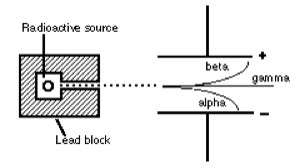
\includegraphics[width=150px]{/Users/shauryasingh/org/chem/images/rayplatediagram.png}
\end{center}

\item Incineration does not decrease radioactivity. Burning nuclear waste will
contaminate the surrounding air, making it deadly
\end{enumerate}

\section{How many moles are in a sample of 300 atoms of Nitrogen (N)? How many grams?}
\label{sec:org99de753}
One mole contains \(6.022 *10^{23}\) atoms, or Avogadro's number. As a result, 300 atoms of nitrogen contain:
\begin{align*}
n&=300\ atoms\\
&=\frac{300}{6.022*10^{23}}\ \frac{atoms}{mol}\\
&=5*10^{-22}\ mol
\end{align*}
Therefore, there are \(5*10^{-22}\ mol\) in 300 atoms of Nitrogen. To calculate
for mass, we multiply the molar mass by the number we calculated earlier
\(14.007 \frac{g}{mol}\times5*10^{-22}\ mol=7*10^{-21}\)
Therefore, 300 atoms of nitrogen contain \(7*10^{-21}g\) of nitrogen.

\section{A sample of sulfur (S) has a mass of 5.37 g. How many moles are in the sample? How many atoms?}
\label{sec:org65d995b}
Sulfur has a molar mass of 32amu. Therefore, it has a molar mass of
\(32\frac{g}{mol}\)
With that information we can make the following equation:
\begin{align*}
\frac{5.37g}{32g/mol}&=0.1678mol\\
&\approx0.17mol
\end{align*}
To convert that to atoms, we can use Avogadro's number (\(6.022 *10^{23}\)).
\begin{align*}
x&=(6.022*10^{23})*(0.17)\\
&=1.02374*10^{23}\\
&\approx1.0*10^{23}
\end{align*}
Therefore there are \(0.17mol\) and \(1.0\times10^{23}\) atoms in the sample of sulfur

\section{How many grams of zinc are in 1.16 x 10 22 atoms of zinc (Zn)?}
\label{sec:org93c32b5}
Zinc atoms have a mass of 65.4g. Using Avagadro's number, we know that there are \(6.022 *10^{23}\) atoms per mole of zinc.
We also know Zinc has a molar mass of \(65.4\frac{g}{mol}\)
From that we can get the following formula
\begin{align*}
x&=\frac{1.16*10^{22}}{6.022*10^{23}}\times65.4 \frac{g}{mol}\\
&=0.0192mol\times65.4\frac{g}{mol}\\
&=1.25568g\\
&\approx1.26g
\end{align*}
Therefore, there are 1.26 grams of zinc in \(1.16\times10^{22}\) atoms  of zinc

\section{Calculate the number of grams per mole (gfm) for each of the following:}
\label{sec:org96969ac}
\begin{enumerate}[(a)]
\item What is the gfm of \(\ce{CuSO4}\)

To find the molar mass of \(\ce{CuSO4}\), we must take the molar mass of
each element in the molecule, and add it together.

\(\ce{Cu}\) (Copper) has a molar mass of 63.546 g/mol.

\(\ce{S}\) (Sulfur) has a molar mass of 32.065 g/mol.

\(\ce{O}\) (Oxygen) has a molar mass of 16 g/mol. Since we have 4 oxygen
atoms, the actual molar mass would be \(16*4=64\) g/mol

Combining the molar mass of the 3 elements, we get
\begin{align*}
63.546+64+32.065=159.611\ g/mol
\end{align*}

\item What is the gfm of \(\ce{NH4OH}\)

To find the molar mass of \(\ce{NH4OH}\) we must take the molar mass of each element in the molecule, and add it together.

\(\ce{N}\) (Nitrogen) has a molar mass of 14.0067 g/mol.

\(\ce{O}\) (Oxygen) has a molar mass of 15.9994 g/mol.

\(\ce{H}\) (Hydrogen) has a molar mass of 1.00794 g/mol. Since we have 5
Hydrogen molecules, that means the molar mass for this element will be
\(1.0088*5=5.0397\ g/mol\).

Combining the molar mass of the 3 elements, we get
\begin{align*}
14.0067+15.9994+1.00794=35.04580\ g/mol
\end{align*}

\begin{enumerate}
\item What is the gfm of \(\ce{Zr(SeO3)2}\)

To find the molar mass of \(\ce{NH4OH}\) we must take the molar mass of each element in the molecule, and add it together.

\(\ce{Zr}\) (Zirconium) has a molar mass of 91.224 g/mol.

\(\ce{O}\) (Oxygen) has a molar mass of 15.9994 g/mol. Since we have 6
Oxygen molecules, that means the molar mass for this element will be
\(15.9994*6=95.9964\ g/mol\).

\(\ce{Se}\) (Selenium) has a molar mass of 78.971 g/mol. Since we have 2
Selenium molecules, that means the molar mass for this element will be
\(78.971*2=157.92\ g/mol\).

Combining the molar mass of the 3 elements, we get
\begin{align*}
91.224+157.92+95.9964=345.16\ g/mol
\end{align*}
\end{enumerate}

\item What is the gfm of \(\ce{Ca2Fe(CN)6*12H2O}\)

 To find the molar mass of \(\ce{Ca2Fe(CN)6*12H2O}\) we must take the molar
mass of each element in each molecule, and add it together.

\(\ce{Ca}\) (Calcium) has a molar mass of 40.087 g/mol. Since there are two
  \(\ce{Ca}\) atoms, we multiply that by two to get 80.174 g/mol

\(\ce{Fe}\) (Iron) has a molar mass of 55.845 g/mol.

\(\ce{C}\) (Carbon) has a molar mass of 12.0107 g/mol. Since we have 6
Carbon molecules, that means the molar mass for this element will be
\(12.0107*6=72.0642\ g/mol\).

\(\ce{N}\) (Nitrogen) has a molar mass of 14.0067 g/mol. Since we have 6
Nitrogen molecules, that means the molar mass for this element will be
\(14.0067*6=84.0402\ g/mol\).

\(\ce{H}\) (Hydrogen) has a molar mass of 1.00794 g/mol. Since we have 24
Hydrogen molecules, that means the molar mass for this element will be
\(1.00794*24=24.19056\ g/mol\).

\(\ce{O}\) (Oxygen) has a molar mass of 15.9994 g/mol. Since we have 12
Oxygen molecules, that means the molar mass for this element will be
\(15.9994*12=191.9928\ g/mol\).

Combining the molar mass of the 2 molecules, we get
\begin{align*}
80.174+55.845+72.0642+84.0402+24.19056+191.9928=508.307\ g/mol
\end{align*}
\end{enumerate}

\section{How many moles of cadmium bromide (\(\ce{CdBr2}\)) are in a 39.25 g sample?}
\label{sec:org6cad2af}
For this we can use Avogadro's number. One mole contains \(6.022*10^{23}\) particles. From that we get the following
\begin{align*}
&N = molar\ mass\\
&No = 272.219\\
&n = moles\\
&n=\frac{N}{No}
\end{align*}
Therefore, we can get
\begin{align*}
n&= \frac{39.25}{272.219}\\
&=0.144185380153\\
&\approx0.144
\end{align*}
Rounding to 4 significant figures, there will be \(1.44*10^-1\) moles of cadmium bromide in a 39.25 g sample

\section{\(\ce{CH3CH2OH}\) boils at 78 °C and \(\ce{CH3OCH3}\) boils at - 24 °C, although both compounds have the same composition. This difference in boiling points may be attributed to a difference in}
\label{sec:orgab8fd02}
The answer is \textbf{D}. Hydrogen bonding. The extra hydrogen bonds of \(\ce{CH3CH2OH}\) make it harder to separate molecules, as more heat and energy is required, resulting in a higher boiling point compared to \(\ce{CH3OCH3}\)

\section{Which of the following elements has the smallest ionization energy? Explain.}
\label{sec:org49f0bee}
Ionization energy decreases down a group, and increases from left to right
across a period. Therefore, Potassium has the smallest ionization energy, which is \textbf{D}.

\section{Which of the following represents the ground state electron configuration for the Mn 3+ ion? (Atomic number Mn = 25) (Hint: first write the e - config of Mn atom, then try the Mn 3+ ion.)}
\label{sec:org04b1270}
The electron configuration for \(\ce{Mn}\) is \(\ce{1s^2 2s^2 2p^6 3s^2 3p^6 3d^5 4s^2}\). The 3+ ion will have 3 fewer electrons, since a positive charge indicates more protons than electrons. Therefore, the electron configuration of \(\ce{Mn^{3+}}\) is \(\ce{1s^2 2s^2 2p^6 3s^2 3p^6 3d^4}\), and the correct option is \textbf{C}

\section{Which of the following represents an excited state?}
\label{sec:orgaf3fbb6}
Option \textbf{D}, \(\ce{1s^2 2s^2 2p^6 3s^2 3p^6 3d^4 4s^2}\) is in an excited state, as it skips the final electron in the 3d orbital.

\section{The table above shows the first three ionization energies for atoms of four elements from the third period of the periodic table. Answer the following questions.}
\label{sec:org3775e52}
\begin{enumerate}[(a)]
\item What is the chemical symbol for element 3, explain your reasoning.
 The third element is \(\ce{Mg}\), or Magnesium. It has low first and second
ionization energies relative to the third, which means it has two valence
electrons. Magnesium is the element with two valence electrons in the third
period of the periodic table

\item Write the complete electron configuration of element 3.
 \(\ce{Mg}\) has an atomic number of 12, therefore the electron configuration
of Magnesium is \(\ce{1s^2 2s^2 2p^6 3s^2}\)

\item What is the chemical symbol for element 2 and what is the expected ion charge for its most common ion?
 The symbol for element 2 is \(\ce{Na}\), and the expect ion charge for its
most common ion is 1+.

\item A neutral atom of which of the four elements above has the smallest radius? Write the symbol for this element and explain this using the first ionization values given.
Element 1 \(\ce{Cl}\), Atomic radius has a trend from right to left across a period, while ionization energy has a trend from left to right across a period. Since element 1 has the highest ionization energy, it would have the smallest atomic radius

\item Which would have a higher electronegativity, element 1 or 4? Briefly explain.
Element 1 would have a higher electronegativity. Both electronegativity and ionization energy follow the same trend, this means that the element with the higher ionization energy will have a higher electronegativity. In this case, that is element 1.

\item The elements are \(\ce{Cl}\), \(\ce{Na}\), \(\ce{Mg}\), and \(\ce{S}\) respectively.
\end{enumerate}

\section{Calculate the mass percent of \(\ce{Cl}\) in each of the following compounds}
\label{sec:org092fe0f}
\begin{enumerate}[(a)]
\item \(\ce{Cl}\)  has a Mass Percent of \%\(65.110\) in \(\ce{CIF}\)
\item \(\ce{Cl}\)  has a Mass Percent of \%\(51.787\) in \(\ce{HClO2}\)
\item \(\ce{Cl}\)  has a Mass Percent of \%\(52.737\) in \(\ce{CuCl2}\)
\end{enumerate}

\section{Calculate the mass percent of each element in \(\ce{Ba(OH)2*8H2O}\), or barium hydroxide octahydrate}
\label{sec:org2db4581}
\begin{enumerate}[(a)]
\item \(\ce{Ba}\)  has a Mass Percent of \%\(43.532\) in \(\ce{Ba(OH)2*8H2O}\),
\item \(\ce{H}\)  has a Mass Percent of \%\(5.751\) in \(\ce{Ba(OH)2*8H2O}\),
\item \(\ce{O}\)  has a Mass Percent of \%\(50.717\) in \(\ce{Ba(OH)2*8H2O}\),
\end{enumerate}

\section{A compound is found, by mass spectral analysis, to contain the following percentages of elements by mass, C = 49.67\%, Cl = 48.92\%, H = 1.39\%, The molar mass of the compound is 289.9 g/mole. Determine the empirical and molecular formulas of the compound.}
\label{sec:orge555358}
\begin{align*}
&C:\ \frac{49.67g}{1}\times\frac{1mol\ce{S}}{12.01g}=4.135mol\\
&Cl:\ \frac{48.92g}{1}\times\frac{1mol\ce{Cl}}{35.453g}=1.380mol\\
&H:\ \frac{1.39g}{1}\times\frac{1mol\ce{H}}{1.008g}=1.380mol\\
&E.F.M.=(3)12.011g+35.453g+1.008g=72.494g
\end{align*}
From that we can calculate the following ratios:
\begin{align*}
&\frac{4.135mol}{1.380mol}=3\\
&\frac{1.380mol}{1.380mol}=1\\
&\frac{1.380mol}{1.380mol}=1
\end{align*}
Since \(\ce{C}\), \(\ce{Cl}\), and  \(\ce{H}\) have a ratio of \(3:1:1\), the molecular formula will be \(\ce{(C3ClH)_n}\) To calculate the empirical formula we solve for n
\begin{align*}
n&=\frac{289.9g}{72.494g}\\
&=4
\end{align*}
Therefore, we can substitute 4 for n.
\begin{align*}
\ce{(C3ClH)_n}&=\ce{(C3ClH)4}\\
&=\ce{C12Cl4H4}
\end{align*}

\section{Determine the empirical formula of a compound that contains the following percentages of elements by mass: Mo = 43.95\%, O = 7.33\%, Cl = 48.72\%.}
\label{sec:orged83f3c}
\begin{align*}
&Mo:\ \frac{43.95g}{1}\times\frac{1mol\ce{Mo}}{95.95g}=0.458mol\\
&Cl:\ \frac{48.72g}{1}\times\frac{1mol\ce{Cl}}{35.45g}=1.374mol\\
&O:\ \frac{7.33g}{1}\times\frac{1mol\ce{O}}{15.99g}=0.458mol
\end{align*}
From that we can calculate the following ratios:
\begin{align*}
&\frac{0.458mol}{0.458mol}=1\\
&\frac{1.374mol}{0.458mol}=3\\
&\frac{0.458mol}{0.458mol}=1
\end{align*}
 Since \(\ce{Cl}\), \(\ce{Mo}\), and  \(\ce{O}\) have a ratio of \(3:1:1\), the
emperical formula will be  \(\ce{Cl3MoO}\)

\section{Aspartame is an artificial sweetener used in food and beverages that is 160 times sweeter than sucrose.}
\label{sec:orgd52d7d1}
\begin{enumerate}[(a)]
\item Using the molecular structure, determine the molecular formula of aspartame,
using this format \(\ce{C_{W}H_{X}N_{Y}O_{Z}}\)

\textbf{Answer:} There are 18 hydrogen atoms, 14 Carbon atoms, 2 Nitrogen atoms, and 5 Oxygen atoms. Therefore, the solution is \(\ce{C14H18N2O5}\)
\item How many molecules are present in 10.0 mg of aspartame? How many hydrogen atoms? O atoms?
\(14\times6+18\times1+2\times7+5\times8=283\frac{g}{mol}\)
\begin{align*}
mol&=\frac{g}{g/mol}\\
mol&=\frac{10g}{283g/mol}\\
mol&=0.035
\end{align*}
Therefore, there are \(0.035mol\) of aspartame in 10 grams
Multiplied by Avogadro's number, that's \(2.05*10^{22}\) molecules.

\item There is \(4.9*10^{-22}g\) in \(1.0*10^{9}\) molecules of aspartame. There
is \(4.9*10^-22g\) in 1 molecule of aspartame
\end{enumerate}

\section{Watch the following video on making a solution and how to calculate molarity and answer the following questions:}
\label{sec:orge93bc9b}
\begin{enumerate}[(a)]
\item Describe how you would make 100.0 mL of a 1.0 M solution of lithium chloride.
\end{enumerate}
We have a \(1.0M\) solution, which translates to  a \(1.0mol/L\)
We need to find the value for \(100ml\), or \(0.1L\)
\(y = 100mL = 0.1L\)
We can plug that into this equation, and solve for x
\begin{align*}
x&= M * y(mol/L) * LiCl\frac{g}{mol}\\
&1.0 * 0.1(mol/L) * 42.394\frac{g}{mol}\\
&0.1mol * 42.394\frac{g}{mol}\\
&4.2394g\\
\end{align*}
Therefore, in order to get 100mL of lithium chloride, we must need 4.2394g of lithium chloride
\begin{enumerate}
\item First we must get our lithium chloride.
\item Afterwards, using our electronic balance, lab scoop, and weighing paper we can measure out 4.2394g of LiCl.
\item Once we calculate that out, we can use a 100.0mL volumetric flask to measure it.
\item Since the molarity is \(1.0mol/L\), 100\% of the solution is \(\ce{LiCL}\), and no
water is required.
\end{enumerate}
\begin{enumerate}
\item Design an experiment to collect data that supports the claim that your 100.0 mL, 1.0 M LiCl solution is a homogeneous mixture.
\begin{enumerate}
\item First we transfer the solution to a 100mL beaker
\item Now, we will heat this solution until it boils and water starts
evaporating. We will place a cold surface above the steam coming out from
the boiling solution.
\item What we will observe is that when all the water evaporates, we can see
white precipitate of NaCl in the bottom of the container. We will also
see that water has condensed on the sides of the container
\item We used physical methods to restore the components of the solution
separately. Based on these observations, we prove that \(\ce{NaCl}\) is a
homogenous solution
\end{enumerate}
\end{enumerate}

\section{The structures of a water molecule and a crystal of LiCl(s) are represented above. A student prepares a 0.10 M solution by dissolving LiCl(s) in enough water to make 100.0 mL of solution.}
\label{sec:orgf917132}
\begin{enumerate}[(a)]
\item How much LiCl(s) was dissolved to make the 0.10 M solution? Justify with a
calculation.
\begin{enumerate}
\item We have a \(0.10M\) solution, which translates to  a \(0.10mol/L\)
We need to find the value for \(100ml\), or \(0.1L\)
\(y = 100mL = 0.1L\)
We can plug that into this equation, and solve for x
\begin{align*}
x&= M * y(mol/L) * LiCl\frac{g}{mol}\\
&0.10 * 0.1(mol/L) * 42.394\frac{g}{mol}\\
&0.01mol * 42.394\frac{g}{mol}\\
&0.42394g\\
\end{align*}
Therefore, \(0.42394g\) of \(\ce{LiCl}\) was dissolved to make the solution
\end{enumerate}

\item Show the interactions of the components of LiCl(aq) by making a drawing.
\end{enumerate}
\begin{center}
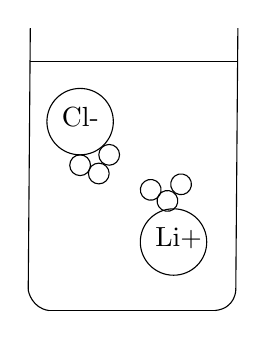
\begin{tikzpicture}[x=0.75pt,y=0.75pt,yscale=-1,xscale=1]
\draw    (201,34) -- (200,160) ;
\draw    (301,34) -- (300,160) ;
\draw    (210,170) -- (290,170) ;
\draw    (200,160) .. controls (200,161) and (202,169) .. (210,170) ;
\draw    (300,160) .. controls (300,160) and (300,169) .. (290,170) ;
\draw    (201,50) -- (301,50) ;
\draw   (209,79) .. controls (209,70.16) and (216.16,63) .. (225,63) .. controls (233.84,63) and (241,70.16) .. (241,79) .. controls (241,87.84) and (233.84,95) .. (225,95) .. controls (216.16,95) and (209,87.84) .. (209,79) -- cycle ;
\draw   (254,137) .. controls (254,128.16) and (261.16,121) .. (270,121) .. controls (278.84,121) and (286,128.16) .. (286,137) .. controls (286,145.84) and (278.84,153) .. (270,153) .. controls (261.16,153) and (254,145.84) .. (254,137) -- cycle ;
\draw   (220,100) .. controls (220,97.24) and (222.24,95) .. (225,95) .. controls (227.76,95) and (230,97.24) .. (230,100) .. controls (230,102.76) and (227.76,105) .. (225,105) .. controls (222.24,105) and (220,102.76) .. (220,100) -- cycle ;
\draw   (234,95) .. controls (234,92.24) and (236.24,90) .. (239,90) .. controls (241.76,90) and (244,92.24) .. (244,95) .. controls (244,97.76) and (241.76,100) .. (239,100) .. controls (236.24,100) and (234,97.76) .. (234,95) -- cycle ;
\draw   (229,104) .. controls (229,101.24) and (231.24,99) .. (234,99) .. controls (236.76,99) and (239,101.24) .. (239,104) .. controls (239,106.76) and (236.76,109) .. (234,109) .. controls (231.24,109) and (229,106.76) .. (229,104) -- cycle ;
\draw   (254.08,111.05) .. controls (254.52,108.33) and (257.1,106.48) .. (259.82,106.93) .. controls (262.55,107.37) and (264.39,109.94) .. (263.95,112.67) .. controls (263.5,115.39) and (260.93,117.24) .. (258.2,116.8) .. controls (255.48,116.35) and (253.63,113.78) .. (254.08,111.05) -- cycle ;
\draw   (268.7,108.38) .. controls (269.15,105.66) and (271.72,103.81) .. (274.44,104.26) .. controls (277.17,104.7) and (279.02,107.28) .. (278.57,110) .. controls (278.12,112.73) and (275.55,114.57) .. (272.83,114.13) .. controls (270.1,113.68) and (268.25,111.11) .. (268.7,108.38) -- cycle ;
\draw   (262.13,116.38) .. controls (262.58,113.66) and (265.15,111.81) .. (267.87,112.26) .. controls (270.6,112.7) and (272.45,115.27) .. (272,118) .. controls (271.55,120.73) and (268.98,122.57) .. (266.26,122.13) .. controls (263.53,121.68) and (261.68,119.11) .. (262.13,116.38) -- cycle ;
\draw (215,71) node [anchor=north west][inner sep=0.75pt]   [align=left] {Cl-};
\draw (260,129) node [anchor=north west][inner sep=0.75pt]   [align=left] {Li+};
\end{tikzpicture}
\end{center}
\end{document}
